\baselineskip=8mm
% \renewcommand{\thesubsection}{\thechapter.\arabic{subsection}}
\numberwithin{equation}{chapter}
\numberwithin{equation}{section}
\renewcommand{\thesubsection}{\arabic{subsection}.}
\renewcommand{\theequation}{\thesection.\arabic{equation}}
\renewcommand{\thesection}{}
\renewcommand{\thesubsubsection}{\thesubsection\arabic{subsubsection}.}




\section{การออกแบบหน้าจอแสดงผล}

%add figure
% \begin{figure}[h]
%     \centering
%     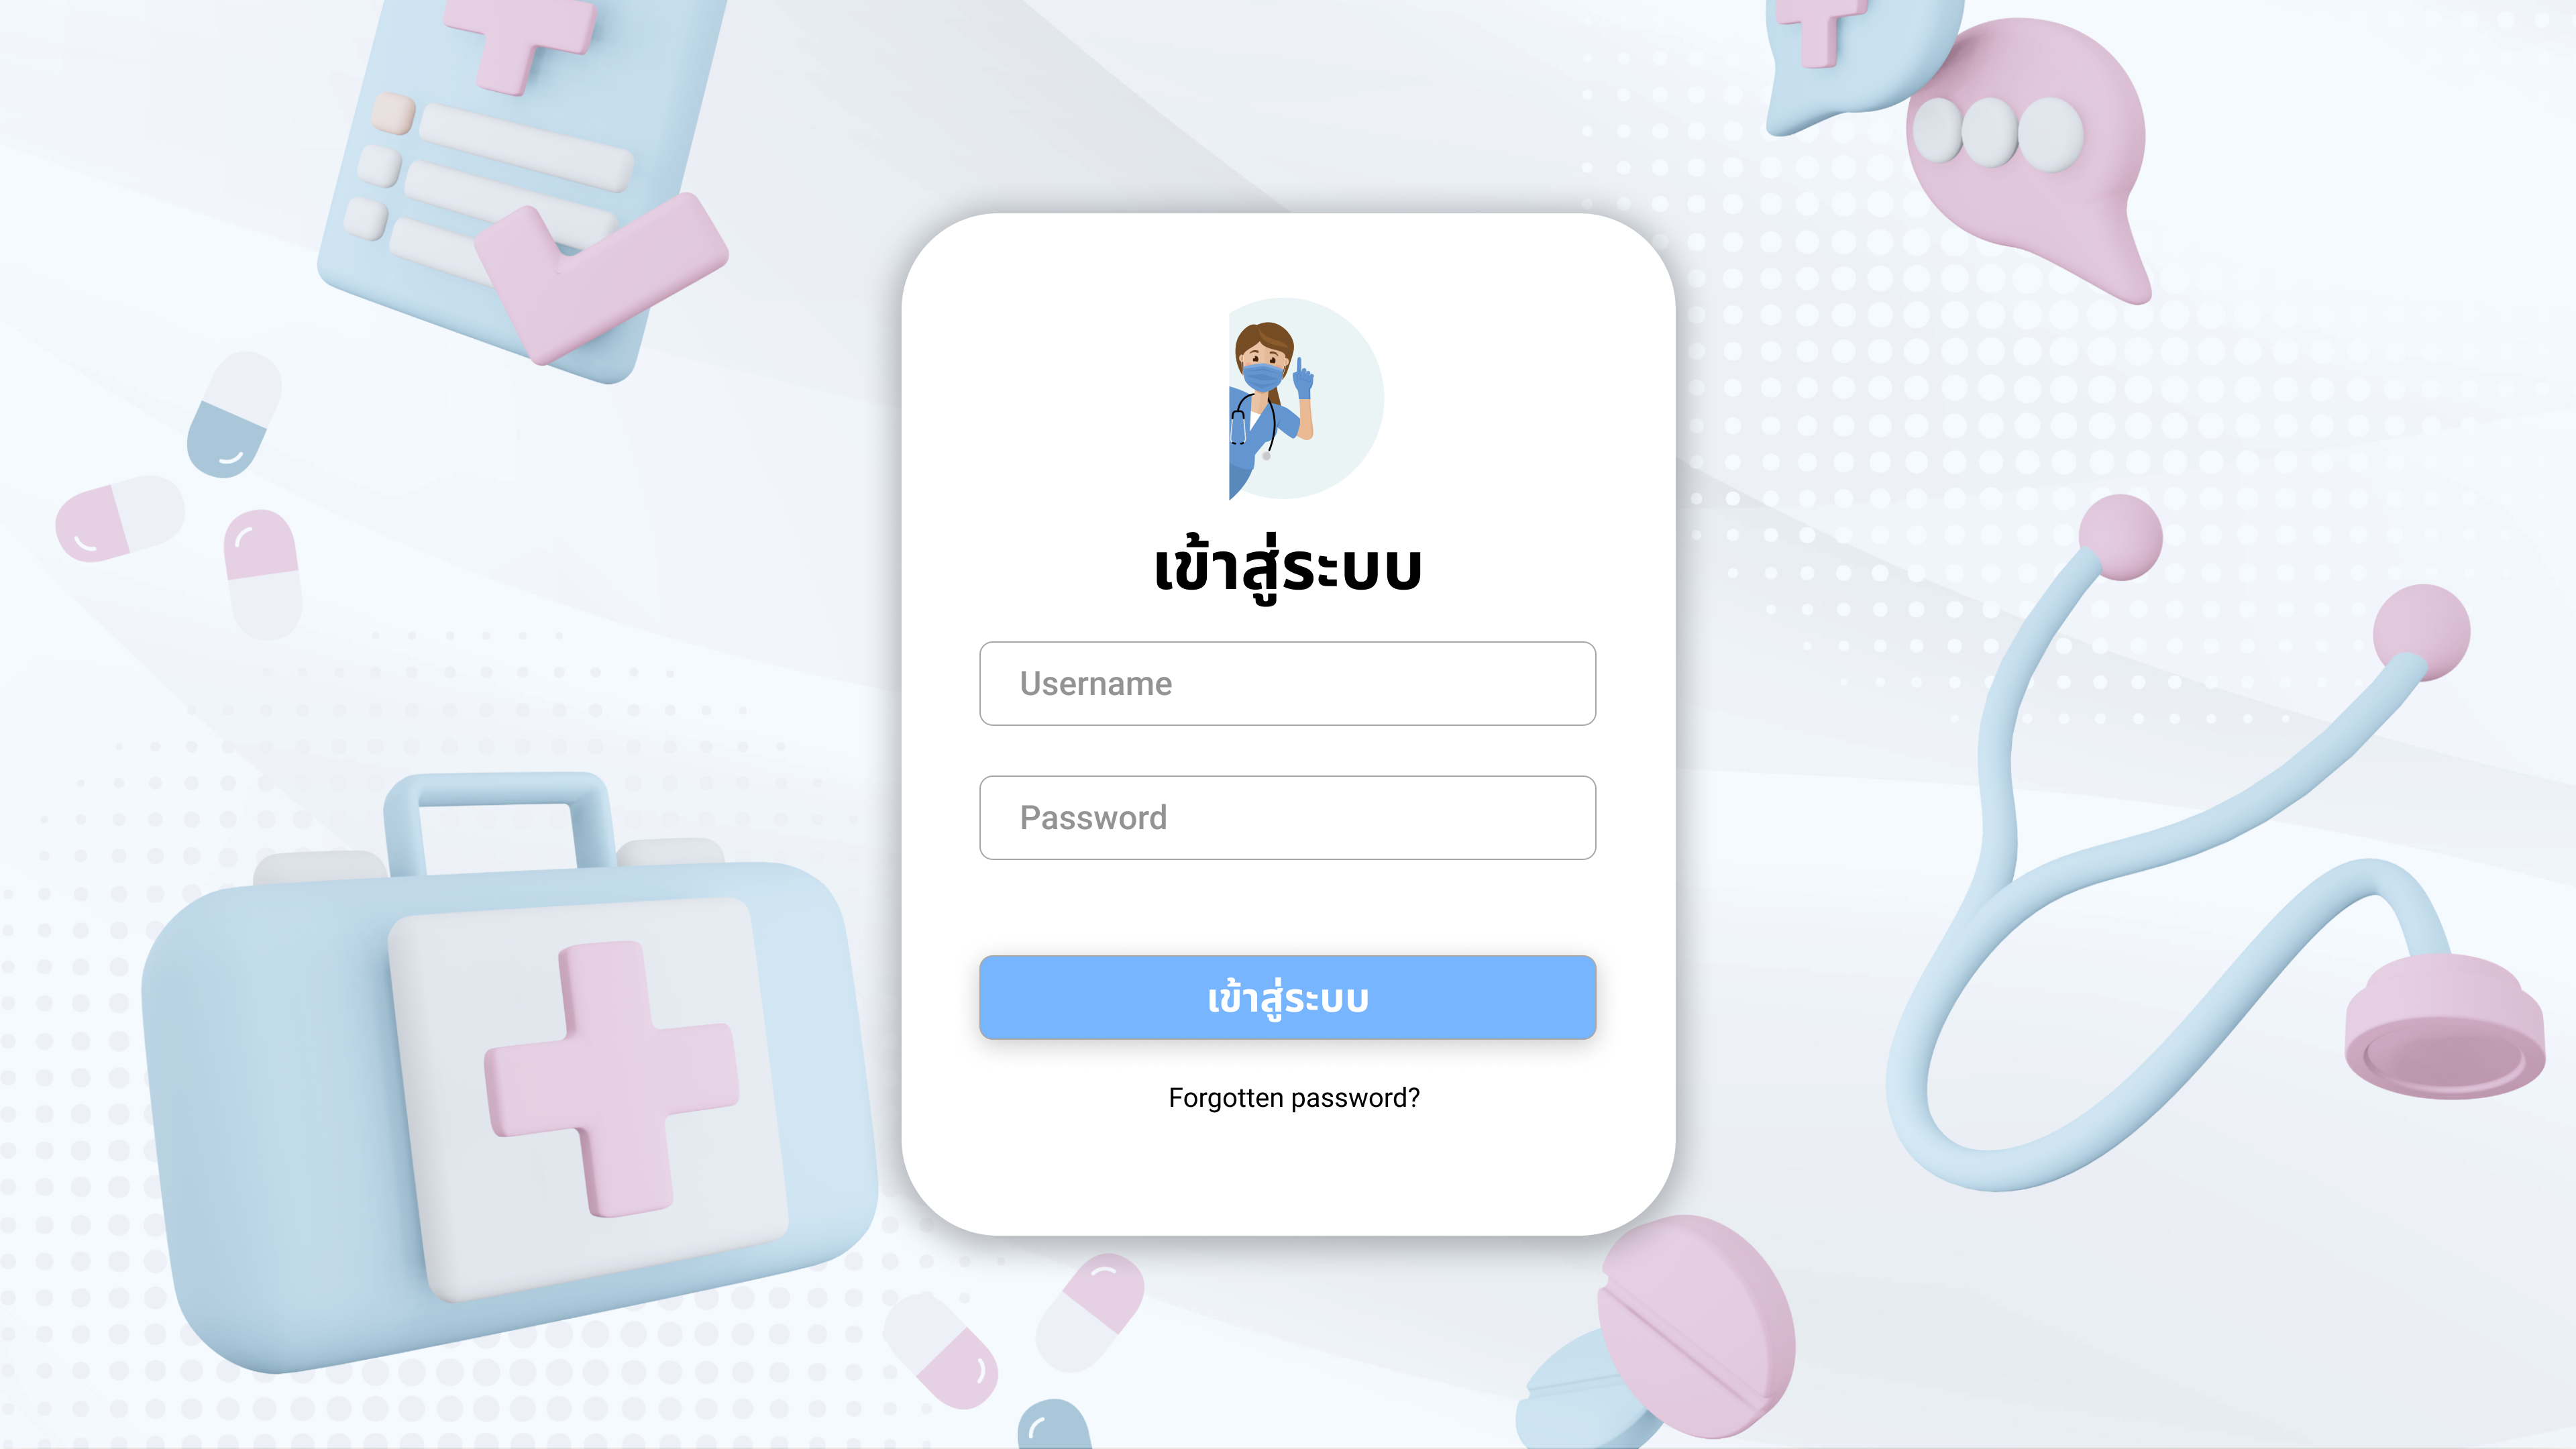
\includegraphics[width=0.6\textwidth]{Login ui.png}
%     \caption{Login}
%     \end{figure}


\subsection{User 1}

\subsection{User 2}

\subsection{User 3}

\subsection{User 4}

\subsection{User 5}

